\begin{figure}[H]
    \centering

    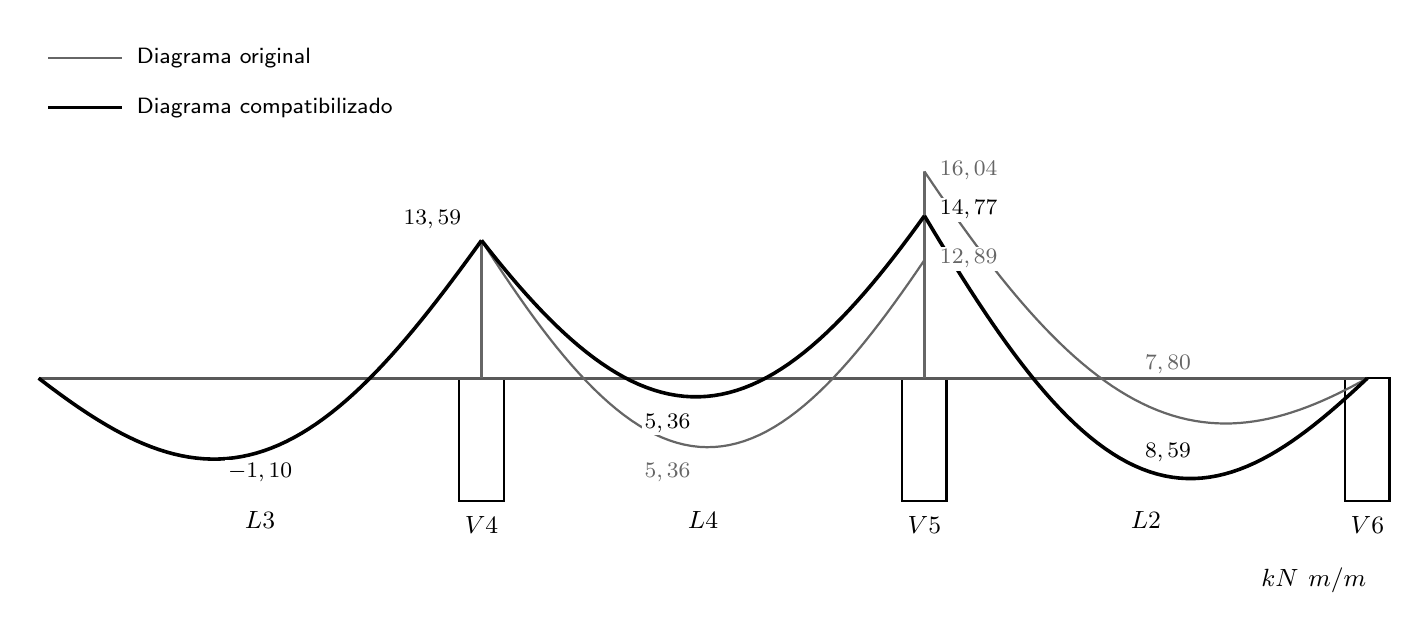
\begin{tikzpicture}[
        scale=1.25,
        pilar/.style={draw=black, thick, fill=white},
        viga/.style={line width=1pt, gray!70!black},
        linhaOriginal/.style={thick, gray!80!black},
        linhaCompat/.style={line width=1.3pt, black},
        cota/.style={<->, >=stealth, thin, black},
        chamada/.style={gray!50, thin, dashed}
    ]

        % --- Parâmetros de Geometria ---
        \def\L{4.5} % Comprimento de cada vão
        \def\Mneg{1.4} % Altura (desenho) do momento negativo em V4 (igual original/compat.)

        % Coordenadas dos Apoios/Pilares
        \coordinate (P0) at (-\L, 0);
        \coordinate (P1) at (0, 0);
        \coordinate (P2) at (\L, 0);
        \coordinate (P3) at (2*\L, 0);

        % 1. Desenho dos 4 Pilares
        \def\wP{0.45}
        \def\hP{1.25}

        % Pilar 0 (x = -L) -- NOVO
        %\draw[pilar] (-\L-\wP/2, -\hP) rectangle (-\L+\wP/2, 0);
        %\node[below=2pt, font=\small\bfseries] at (-\L, -\hP) {$V3$};

        % Pilar 1 (x = 0)
        \draw[pilar] (-\wP/2, -\hP) rectangle (\wP/2, 0);
        \node[below=2pt, font=\small\bfseries] at (0, -\hP) {$V4$};

        % Pilar 2 (x = L)
        \draw[pilar] (\L-\wP/2, -\hP) rectangle (\L+\wP/2, 0);
        \node[below=2pt, font=\small\bfseries] at (\L, -\hP) {$V5$};

        % Pilar 3 (x = 2L)
        \draw[pilar] (2*\L-\wP/2, -\hP) rectangle (2*\L+\wP/2, 0);
        \node[below=2pt, font=\small\bfseries] at (2*\L, -\hP) {$V6$};

        % 2. Eixo das Vigas (agora de -L a 2L)
        \draw[viga] (-\L, 0) -- (2*\L, 0);

        % Rótulos das Vigas no Centro de Cada Vão (Parte Inferior)
        \node[below=2pt, font=\small\bfseries, fill=white, inner sep=1.5pt] at (-\L/2, -\hP) {$L3$};
        \node[below=2pt, font=\small\bfseries, fill=white, inner sep=1.5pt] at (\L/2, -\hP) {$L4$};
        \node[below=2pt, font=\small\bfseries, fill=white, inner sep=1.5pt] at (1.5*\L, -\hP) {$L2$};

        \node[right, font=\small\bfseries, fill=white, inner sep=1.5pt] at (1.75*\L, -\hP-0.8) {$kN \ m/m$};

    % CHAMADA MEIO

    % --- C. LINHAS VERTICAIS NOS PILARES ---
    \coordinate (Pt1) at (\L, 1.2);   % Ponto do diagrama original V1
    \coordinate (Pt2) at (\L, 1.65);  % Ponto do diagrama compatibilizado
    \coordinate (Pt3) at (\L, 2.1);   % Ponto do diagrama original V2

    \draw[line width=1pt, gray!80!black] (\L, 0) -- (Pt3);

    % Linha vertical em V4 (momento negativo igual no original e no compatibilizado)
    \draw[line width=1pt, gray!80!black] (0, 0) -- (0, \Mneg);

    % 3. DIAGRAMA DE MOMENTOS FLETORES

    % --- NOVO VÃO L0 (-L a 0): original = compatibilizado ---
    \draw[linhaOriginal]
        plot[domain=-\L:0, samples=60] (\x, {-1.10 * sin((\x+\L) * 180 / \L) + \Mneg * ((\x+\L)/\L)^2});
    \draw[linhaCompat]
        plot[domain=-\L:0, samples=60] (\x, {-1.10 * sin((\x+\L) * 180 / \L) + \Mneg * ((\x+\L)/\L)^2});

    % --- A. Linha Original (Antes da Compatibilização) ---
    % Vão 1 (0 a L): agora com momento negativo também em x=0
    \draw[linhaOriginal]
        plot[domain=0:\L, samples=60] (\x, {-1.35 * sin(\x * 180 / \L) + 1.2 * (\x/\L)^2 + \Mneg * ((\L-\x)/\L)^2});

    % Vão 2 (L a 2L)
    \draw[linhaOriginal]
        plot[domain=\L:2*\L, samples=60] (\x, {-0.8 * sin((\x-\L) * 180 / \L) + 2.1 * ((2*\L-\x)/\L)^2});

    % --- B. Linha Compatibilizada (Após a Compatibilização) ---
    % Vão 1
    \draw[linhaCompat]
        plot[domain=0:\L, samples=60] (\x, {-0.95 * sin(\x * 180 / \L) + 1.65 * (\x/\L)^2 + \Mneg * ((\L-\x)/\L)^2});

    % Vão 2
    \draw[linhaCompat]
        plot[domain=\L:2*\L, samples=60] (\x, {-1.35 * sin((\x-\L) * 180 / \L) + 1.65 * ((\x-\L)/\L - 1)^2});

    % 4. RÓTULOS DOS MOMENTOS MÁXIMOS

    % Sobre o Pilar V4 (momento negativo, igual original/compat.) -- NOVO
    \node[above=3pt, font=\sffamily\footnotesize\bfseries, black, fill=white, inner sep=1pt]
        at (-0.5, \Mneg) {$13,59$};

    % No Vão L0 (igual original/compat.) -- NOVO
    \node[below=1pt, font=\sffamily\footnotesize\bfseries, black, fill=white, inner sep=1pt]
        at (-0.5*\L, -0.8) {$-1,10$};

    % Sobre o Pilar P2 (Momentos Negativos):
    \node[above=3pt, font=\sffamily\footnotesize\bfseries, gray!80!black, fill=white, inner sep=1pt]
        at (\L+0.45, 1) {$12,89$};
    \node[above=3pt, font=\sffamily\footnotesize\bfseries, gray!80!black, fill=white, inner sep=1pt]
        at (\L+0.45, 1.9) {$16,04$};

    \node[above=3pt, font=\sffamily\footnotesize\bfseries, black, fill=white, inner sep=1pt]
        at (\L+0.45, 1.5) {$14,77$};

    % No Vão 1 (V1):
    \node[below=1pt, font=\sffamily\footnotesize\bfseries, gray!80!black, fill=white, inner sep=1pt]
        at (0.42*\L, -0.8) {$5,36$};
    \node[below=1pt, font=\sffamily\footnotesize\bfseries, black, fill=white, inner sep=1pt]
        at (0.42*\L, -0.3) {$5,36$};

    % No Vão 2 (V2):
    \node[below=1pt, font=\sffamily\footnotesize\bfseries, gray!80!black, fill=white, inner sep=1pt]
        at (1.55*\L, 0.3) {$7,80$};
    \node[below=1pt, font=\sffamily\footnotesize\bfseries, black, fill=white, inner sep=1pt]
        at (1.55*\L, -0.6) {$8,59$};

        % 5. LEGENDA
        \begin{scope}[shift={(-\L, 3)}]
            \draw[thick, fill=white, draw=white] (-0.1, -0.55) rectangle (3.3, 0.55);
            \draw[linhaOriginal] (0.1, 0.25) -- (0.85, 0.25);
            \node[right, font=\sffamily\footnotesize] at (0.9, 0.25) {Diagrama original};
            \draw[linhaCompat] (0.1, -0.25) -- (0.85, -0.25);
            \node[right, font=\sffamily\footnotesize] at (0.9, -0.25) {Diagrama compatibilizado};
        \end{scope}
    \end{tikzpicture}

    %\caption{Caption}
    %label{fig:placeholder}
\end{figure}